\hypertarget{empiricalModels}{
}

\noindent For the texture synthesis of the materials, various local reflection models can be used\footnote[1]{Another set of reflection models are global illumination models. These are beyond the scope of this thesis.}. This chapter will outline the empirical models used in the process of texture synthesis for the experimental setup. These models capture reflectance behaviour using mathematical models without using any basic laws of physics. Such models are widely used for their simplicity and because they can be controlled by setting only a small set of parameters to obtain desired results. The parameters that need to be set will be obtained by a gradient descend procedure for the experiments; this procedure is explained in section \ref{sec:ParameterSetting}.

\section{Lambertian reflectance}\label{sec:Lambertian}
	One of the most used empirical models is Lambertian reflectance. In computer graphics, this model is mainly used to simulate diffuse reflectance. Surfaces with such properties appear equally bright from all viewing angles because the light is reflected with equal intensity in all directions. The brightness of the surface is only dependent of the angle $\theta_i$ between the surface normal $\vec{\mathbf{n}}$ and the light source direction $\vec{\mathbf{l}}$. 

In general, for Lambertian reflectance, the amount of light observed by the viewer is indepenendent of the viewing angle, and is only dependent on the angle of the incidence of the light source. The full equation is given by:

		\begin{eqnarray*}
			L_o(\omega_i) = \frac{k_d}{\pi}I_p\cos\theta_i
		\end{eqnarray*}

Here, irradiance $E_L$ is defined as $I_p$, the intensity of the point light source, and the BRDF is given by $k_d$, also known as the {\it diffuse reflection coefficient}, which varies between 0 and 1 and is material dependent. The term $\pi$ in the denominator is a normalization factor for energy conservation. The cosine term is defined between $0^0$ and $90^0$. This means that the surface is treated as self-occluding; angles outside this range will result in negative values for the cosine term and are treated as $\max({0,\cos\theta_i})$, resulting in zero intensity falling on the surface. If both $\vec{\mathbf{n}}$ and $\vec{\mathbf{l}}$ are normalized, we can write the equation as:

		\begin{eqnarray*}
			L_o(\omega_i) = \frac{k_d}{\pi}I_p(\vec{\mathbf{n}} \cdot \vec{\mathbf{l}})
		\end{eqnarray*}

This model is used effectively for the synthesis of diffuse surfaces and in interactive software since the reflection term does not need to be recomputed whenever the view changes. However, most materials are deviating from Lambertian for angles of view or incidence greater than $60^0$ \cite{DigitalModeling}. Another shortcoming of Lambertian reflectance is that it does not include the observation of speculars on materials. For these reasons the model is insufficient to synthesize materials with a more glossy/shiny nature since they will need the speculars to be present. In our experiments, we keep the intensity of the point light source constant on $1.0$, and the equation can be simplified more by the removal of $I_p$.

	\section{Phong Reflectance}\label{sec:Phong}
		With the Lambertian assumption of light reflecting equally into all direction, we can expect poor quality synthesis when we are dealing with more glossy/specular surfaces such as metallic and plastic materials. As Bui-Tuong Phong wrote in his article, {\it if the goal in shading a computer-synthesized image is to simulate a real physical object, then the shading model should in some way imitate real physical shading situations} \cite{Phong}. Phong reflectance is a popular model for its broad application in real-time rendering, and is based on the empirical observation of how shiny surfaces can have small specular highlights and how these observed speculars are related to the view direction of the observer.

The general idea of Phong reflection is shown in figure \ref{fig:SPECULAR1}. Here we have an incident angle $\theta_i$ and an equal reflection angle $\theta_r$. The angle between $\vec{\mathbf{r}}$ and $\vec{\mathbf{v}}$, denoted as $\theta_s$, defines how strong a specular is perceived by the observer. If this angle is zero (ie. the reflection- and view-direction are in the same direction), the perceived intensity will be maximal. When this angle increases, the observed intensity of the specular will fall off fast.

\begin{figure}[H]
	\begin{center}
		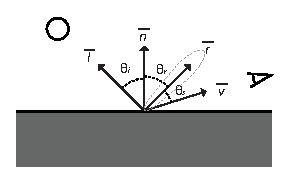
\epsfig{file=images/SpecularReflection.eps, width=0.5\linewidth}
	\end{center}
	\caption{{\it Specular reflection. $\theta_i$ is the angle of the incoming light, and is equal to the reflected angle $\theta_r$. $\theta_s$ is the angle between the view direction and the reflected light.}}
	\label{fig:SPECULAR1}
\end{figure}


\noindent The reflection model is computed as:

	\begin{eqnarray*}
		L_o = (i_a + k_d(\cos\theta_i) + k_s(\cos\theta_s)^\alpha) \otimes E_L
%		L_o = i_a + k_d(\vec{\mathbf{l}} \cdot \vec{\mathbf{n}}) + k_s(\vec{\mathbf{r}} \cdot \vec{\mathbf{v}})^\alpha
	\end{eqnarray*}

\noindent where $i_a$ is a parameter controlling the ambient lighting, $k_d$ is the diffuse reflection coefficient which is material dependent, $k_s$ is the specular reflection coefficient which is also material dependent. The $\alpha$ parameter,also known as the shininess constant, is used to control the size of the specular lobe; the greater $\alpha$ is, the smaller the size of the specular. The angle $theta_i$ is computed by taking the dot product between $\vec{\mathbf{l}}$ and $\vec{\mathbf{n}}$. Likewise, the angle $\theta_s$ is computed by taking the dot product between $\vec{\mathbf{r}}$ and $\vec{\mathbf{v}}$. Vector $\vec{\mathbf{r}}$ is computed such that its mirrored around the surface normal:

	\begin{eqnarray*}
		\vec{\mathbf{r}} = 2 \otimes \vec{\mathbf{n}} \otimes \cos\theta_i - \vec{\mathbf{l}}
	\end{eqnarray*}


%\begin{itemize}
%	\item[] $i_a$ is a parameter controlling the ambient lighting.
%	\item[] $k_d$ is the diffuse reflection coefficient.
%	\item[] $k_s$ is the specular reflection coefficient.
%	\item[] $\vec{\mathbf{l}}$ is the direction vector for the light source.
%	\item[] $\vec{\mathbf{v}}$ is the direction vector for the observer.
%	\item[] $\vec{\mathbf{n}}$ is the surface normal.
%	\item[] $\vec{\mathbf{r}}$ is the direction vector for the reflected light, 
%		calculated as $2\vec{\mathbf{n}}(\vec{\mathbf{l}} \cdot \vec{\mathbf{n}}) - \vec{\mathbf{l}}$
%	\item[] $\alpha$ is a parameter controlling the specular size, also known as the shininess constant, which is material-dependent. The greater $\alpha$ is, the smaller the size of the specular.
%\end{itemize}

%Here, the parameterse $k_d$ and $k_s$ are constants for diffuse and specular reflection respectively. 

The equation for Phong reflectance is simplified such that it does not involve more than one light source. More light sources could be incorporated easily by computing the diffuse and specular components for each light source separately and summing these to obtain the total contribution. With respect to the experiments, multiple light sources are not necessary. Also, the components defining colors are left out since we are only concerned with gray scale images in the experiments. The ambient term can be discarded, since a preprocessing step will make the synthetic images intensity-invariant. A common complaint about the Phong model is that it is completely empirical, and does not abide the most basic law in physics --- the conservation of energy. Appropriate normalization factors could be applied to constrain the model to this law.

	\section{Blinn-Phong Reflectance}\label{sec:BlinnPhong}
		Short after Phong published his model, Blinn proposed an alternative to compute the specular component where the angle $\theta_s$, dot product between the reflection vector and viewing vector, could be replaced by $\theta_h$ \cite{Blinn}. This angle the dot product between the normal of the surface, and the so called halfway-vector $\vec{\mathbf{h}}$. This halfway-vector is the bivector between the light source vector $\vec{\mathbf{l}}$ and the view direction vector $\vec{\mathbf{v}}$, and is computed as:

	\begin{eqnarray*}
		\vec{\mathbf{h}} = \frac{\vec{\mathbf{l}} + \vec{\mathbf{v}}}{|\vec{\mathbf{l}} + \vec{\mathbf{v}}|}
	\end{eqnarray*}

He observed that mirror reflections only occur when the surface normal is aligned with the halfway-vector \cite{DigitalModeling}. When observing a material with glossy/shiny properties, the microscopic structure of the material is never entirely smooth and can be illustrated as microscopic small surfaces. The main normal of the surface is still $\vec{\mathbf{n}}$, but each micro-surface has its own surface normal as well. The distribution of the specular lobe can be expressed as the amount of microfacets with normals aligned with the halfway-vector, with a likelihood related to $\theta_h$.

Replacing $\theta_s$ with $\theta_h$ doesn't give the same reflectance function as with Phong reflection, and as a result it produces slightly different speculars. However, because of computational convenience, Blinn-Phong reflectance is being used in most systems these days.

	\section{Other Models}\label{sec:Other}
		Many other reflection models exists, and they tend to be variations of Phong reflectance. They deal with the conservation of energy, which wasn't addressed by Phong in his original research. An example of a generalization of Phong reflectance is Lafortune reflectance \cite{Lafortune}. This model can produce a BRDF that consists of multiple lobes, and includes a generalized form of diffuse reflectance. In general, diffuse reflectance doesn't reflect radiance uniform over the hemisphere like in the case of Lambertian reflectance, but may peak into the direction of the surface normal and radiance falls off in directions other than that of the surface normal. The model also includes backscatter, the phenomenom of light reflected into the direction of the light source, and it allows for different configurations for the specular lobe (eg. anisotropic or isotropic).

Another modification of Phong reflectance is Ashikhmin-Shirley Anisotropic Phong reflectance \cite{AshikhminShirley}, which includes a Fresnel term in the equations. The model also deals with conservation of energy and allows for anisotropic specular lobes.

While these models can express more BRDFs than the other models described in this chapter, they do need a lot more parameters to be set. Since these parameters are unknown for the materials in this research and are expensive to obtain by computation, these models are left for future research.
